\documentclass[conference]{IEEEtran}
\IEEEoverridecommandlockouts
% The preceding line is only needed to identify funding in the first footnote. If that is unneeded, please comment it out.
\usepackage{cite}
\usepackage{amsmath,amssymb,amsfonts}
\usepackage{algorithmic}
\usepackage{graphicx}
\usepackage{textcomp}
\usepackage{xcolor}
\usepackage{url}
\def\BibTeX{{\rm B\kern-.05em{\sc i\kern-.025em b}\kern-.08em
    T\kern-.1667em\lower.7ex\hbox{E}\kern-.125emX}}
\begin{document}

\title{Hashiko\\
}

\author{\IEEEauthorblockN{1\textsuperscript{st} Jackie Ma}
    \IEEEauthorblockA{\textit{Applied Computer Science} \\
        \textit{British Columbia Institute of Technology}\\
        Burnaby, Canada \\
        jma149@my.bcit.ca}
}

\maketitle

\begin{abstract}
Hashiko is a distributed monitoring system that tracks file integrity and user activity. It detects threats by linking events through time and sequence, such as login, privilege change and file edit. Agents collect data with timestamps and send it to a central server. The server builds event chains and generates alerts. A web interface shows real-time alerts, timelines and rules. The system focuses on accuracy, secure transfer and scalability. Testing uses synthetic data, log replays and simulations to validate components. Scope includes agents, server, storage and interface. Out of scope are malware analysis and compliance reporting. Hashiko improves detection by closing temporal blind spots.
\end{abstract}

\begin{IEEEkeywords}
    agents, central server, distributed monitoring, event chains, event sequencing, file integrity, real-time alerts, rule management, scalability, secure transfer, temporal correlation, timestamped data, user activity, web interface
\end{IEEEkeywords}

\section{Student Background}
I am currently a fourth-year student in the Bachelor of Applied Computer Science program at BCIT, specializing in Network Security Applications Development. Before studying computer science, I studied architecture and briefly worked in the industry. After graduation, I plan to work in software development or IT.

\section{Project Summary}

The project is a distributed monitoring system that tracks both file integrity and user activity. It goes beyond typical IDS tools by detecting threats through timing and sequence patterns. The focus is on temporal relationships. For example, sensitive files being modified right after an unusual login or privilege changes.

Endpoint agents collect file hashes, login sessions and process activity. All data is sent with timestamps to a central server. The server builds time-windowed event chains and flags patterns that isolated event-based systems often overlook. Alerts trigger when suspicious sequences match predefined or custom temporal threat patterns. A web interface provides clear visibility, easy alert tracking and quick access to detailed event data. Thus, the administrator has a centralized and readable view of ongoing risks.

\section{Problem Statement and Background}
Organisations face increasing risks from both external attackers and insider threats. Traditional tools such as intrusion detection systems or file integrity monitors can detect single events. However, they rarely correlate activity over time. Thus, it leaves blind spots where subtle yet dangerous patterns go unnoticed. For example, an unusual login, followed by privilege escalation and then a file change, may seem harmless in isolation but is critical when viewed as a sequence.

The core weakness is the lack of temporal awareness in existing monitoring systems. Timing, order and relationships between events are as important as the events themselves. Without this context, significant risks bypass defences. Visibility is further reduced by scattered logs and rigid dashboards that slow incident response. A centralised system that aggregates events from multiple endpoints, applies timestamps and links them together can close this detection gap. A web interface adds readability by simplifying alert tracking and management.

\section{Inventiveness}

What sets this project apart is its focus on temporal event correlation. Most security tools detect single anomalies, such as a file change or a suspicious login. The project instead looks at the timing and sequence of events across endpoints. It flags patterns that become suspicious only when actions occur together, within specific time windows.

Another inventive aspect is the centralized, distributed design. Endpoint agents collect activity data such as file hashes, logins and processes. Then attach precise timestamps before sending it to the central server. Instead of producing isolated alerts, the system creates linked event chains. A web interface presents these chains in a clear way, giving teams both context and visibility. This blend of distributed data gathering with temporal threat analysis is rarely seen in current monitoring solutions.

\section{Complexity}

The project is complex as the system must collect data from many endpoints and link events in real time with precise timestamps. This makes it significantly more advanced than simple single-event detection. The main challenges include distributed design, synchronisation, secure communication and scaling to handle large data volumes. While a diploma student might build a basic log collector, they would lack the depth to design correlation logic, distributed agents and scalable servers.

The project requires knowledge of network security, analytics and distributed systems. Thus, making it appropriate for a Bachelor student. The most difficult aspect is linking events by time and sequence, which is far more challenging than detecting isolated anomalies. Success requires skills in event processing, threat modelling and testing of correlation models.

\section{Technical Challenges}

The project is technically challenging as it extends beyond the course material. Distributed agents must be designed to securely collect and transmit data, synchronisation and time accuracy across endpoints. A central server will be required to store, process and correlate large event streams in real time, handling event chaining, sequence detection and scaling across multiple hosts.

Another challenge is web development for security monitoring. The interface must present alerts clearly and support custom rule management. Exploration of temporal correlation models and advanced threat detection will be necessary. As these areas are not fully covered in class, industry practices will need to be studied and experimental implementations developed. These factors make the project both demanding and a valuable learning experience.

\section{Methodology and Design}

The project follows an agent–collector–correlator design with a central server and web interface. Agents compute file hashes, monitor file paths, record logins and send timestamped events. The server ingests, validates and stores events. Then the server applies sequence rules to construct time-ordered chains that expose multi-step threats. The web interface delivers real-time alerts, timelines and rule management for rapid triage and investigation.

The methodology combines established even monitoring practices with temporal correlation. Standardised schemas ensure consistent parsing at ingest. Time accuracy is maintained through authenticated synchronisation and drift checks. The correlation engine evaluates ordered predicates within windows, such as unusual login followed by privilege change and then a sensitive write. Optional anomaly baselines strengthen rule-based detection. Storage is indexed by time, entity and file path for fast retrieval. The architecture layers include endpoints, correlation services, durable storage and a clear web interface.

\begin{figure}[h!]
    \centering
    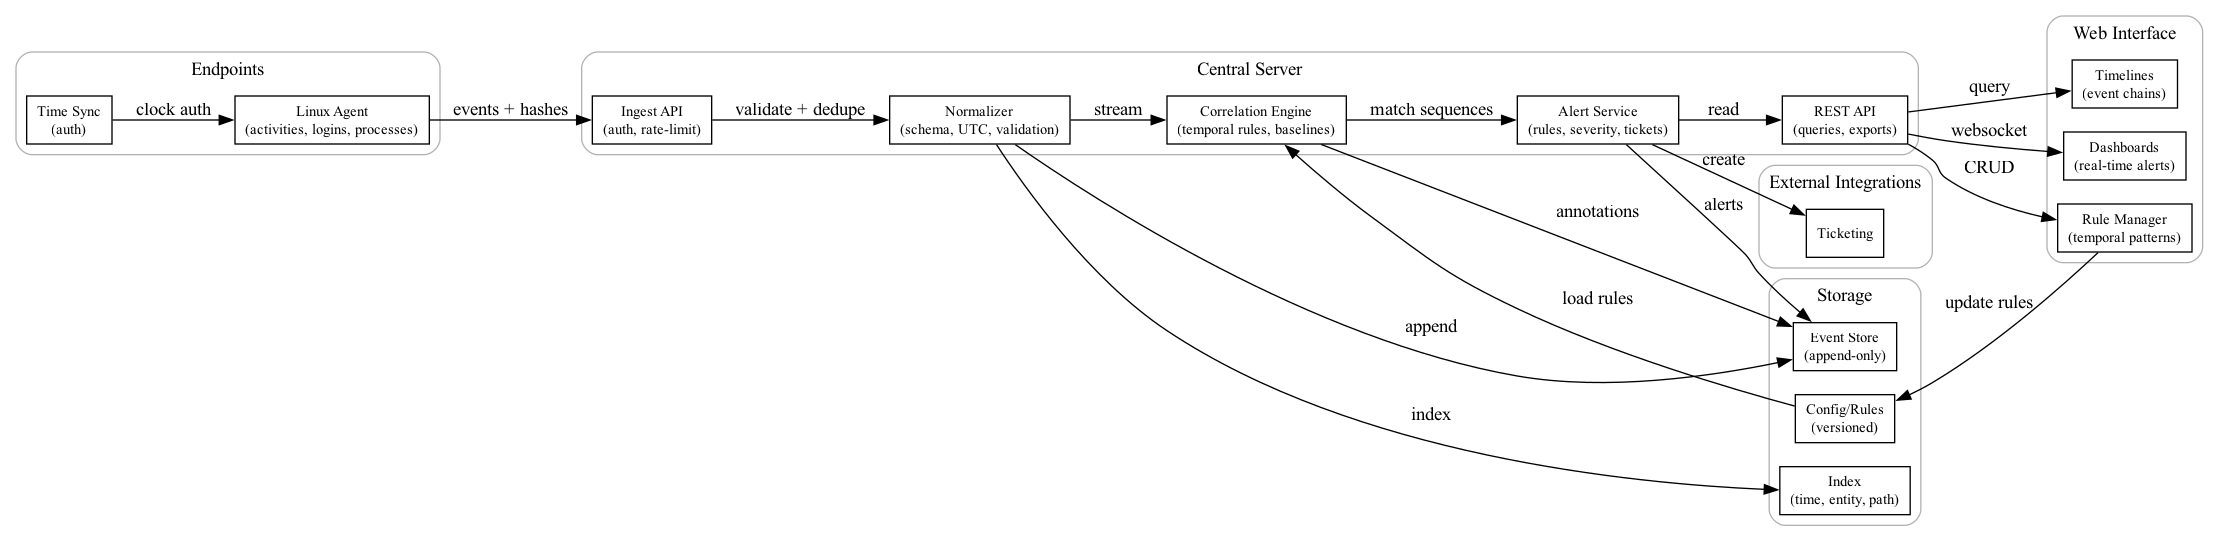
\includegraphics[width=\columnwidth]{../diagrams/systems.png}
    \caption{System Diagram}
    \label{fig:systems}
\end{figure}

\section{Test Plan}

The project will be tested in a staged lab. Synthetic generators, safe log replays and controlled adversarial simulations will be used. These tests will validate agents, transfer, normalization, correlation, storage, APIs and the web interface. Verification uses clear checkpoints for accuracy, throughput, detection latency, durability and UI responsiveness. A release moves forward only when all checkpoints are passed. Agents check files, edits, logins, processes and time. Transfer is tested for loss, replay, order and authentication. Normalization enforces schema and UTC. Correlation measures accuracy, noise and delay. Performance tests speed and scale. Storage checks durability, recovery and search. The interface is tested for alerts, rules, access and stability. End‑to‑end validates visibility, severity, tickets and exports.Scope and Depth
Scope includes agents, a central server, storage and a web interface. Features cover file integrity with baselines and hashes, login and process monitoring, normalised timestamped events, secure transfer, alerts, search and rule management. Deliverables are Linux and one other OS agent, a central pipeline, indexed storage, web interface, documented APIs, starter rules and a test plan.

Out of scope are memory scanning, kernel exploit detection, malware analysis and compliance reports. Depth comes from accurate time sync, sequence-based correlation, scalable ingest, durable storage with replay, explainable rules, timeline views, custom temporal patterns, baseline learning and full security for identity, encryption and audit.

\begin{thebibliography}{00}
    \bibitem{b1} Abdullah, Z. H., Udzir, N. I., Mahmod, R., and Samsudin, K. (2011). File integrity monitor scheduling based on file security level classification. \textit{Communications in Computer and Information Science}, 177--189. \url{https://doi.org/10.1007/978-3-642-22191-0_16}
    \bibitem{b2} Kaczmarek, J., and Wrobel, M. (2008). Modern approaches to file system integrity checking. \textit{2008 1st International Conference on Information Technology}, 1--4. \url{https://doi.org/10.1109/inftech.2008.4621669}
\end{thebibliography}

\end{document}
